%------------------------------------------------- Chapter --------------------------------------------------------
\chapter{arqDHD: Arquitectura de Software para los Dispositivos Hipermediales Dinámicos}\label{cap:arqdhd}

%\pagenumbering{arabic}

\section{Introducción}\label{secc:arqDHD_Introduccion}

En este capítulo se describen los aspectos fundamentales y decisiones adoptadas
en base al tipo de modelos y arquitecturas que se tuvieron en cuenta en el
diseño e implementación de los Dispositivos Hipermediales Dinámicos(DHD).

Esto se logra mediante la caracterización  de algunos aspectos relevantes que se lleva adelante a través de un 
proceso de desarrollo específico para los DHD. Este proceso se destaca por la inclusión
de artefactos derivados, permitiendo caracterizar de manera eficiente aspectos semánticos 
de aquellas componentes de la arquitectura, que juegan un papel importante y permiten
resolver de forma eficaz y eficiente las partes de los requerimientos funcionales de adaptación anteriormente mencionados (sección \ref{requisitoDHD}).

A todas las decisiones de diseño de la arquitectura que se presenta en este capítulo la denominaremos \textbf{arqDHD}  con el propósito de
sentar algunas precedencias hacia el estudio y definición de los procesos de diseño de los \textbf{DHD}. De esta manera, se tuvieron en cuenta diferentes tipos de elementos y criterios de interpretaciones que se ajustan al dominio de aplicación de esta tesis:


\begin{itemize}
 
 \item \textbf{Componentes}: Se refiere a los tipos de componentes que podrán adoptar un rol 
 \textit{cliente}, haciendo peticiones a otros componentes con el rol de \textit{servidores}, encargado de brindar esos servicios. \label{lbl:componente} 
 
 
 \item \textbf{Conectores}: Se refiere a los mecanismos de interacción entre los componentes.
 
 \item \textbf{Contratos}: Es el componente de primera clase, provisto con su propio diseño y funcionalidad que deberá ser inyectado a una arquitectura original.
 
 \item \textbf{Subsistemas}: Se utilizará este concepto para representar la idea de que un sistema externos está conectado con algún componente estructural de la arquitectura. 
 
 \item \textbf{Puertos}:  Son los puntos de conexión entre los componentes. Para este trabajo los puertos que intervienen en las estructuras de inyección de los contratos serán componentes de primera clase.
  
 \item \textbf{Artefactos de penetración}: Encargado de establecer componentes de
composición  o conectores internos de la arquitectura con elementos sus
interfaces externas. 

 \item \textbf{Modelo Computacional Subyacente}: Se refiere a la información necesaria donde se explica el funcionamiento en tiempo de ejecución del sistema que implementa la arquitectura. En este trabajo se utiliza para describir algunas cuestiones semánticas referidas a los mecanismos de inyección de los contratos.


\end{itemize}

Conceptualmente \textbf{arqDHD} está definida por aquellos aspectos de la arquitectura que desempeñan un rol protagónico en los DHD. Esta apreciación fue motivada asumiendo que los
requerimientos de los DHD se deben resolver a partir de la arquitectura sin
tener en cuenta el modo de implementación de aquellos artefactos que la compone.

Además, \textbf{arqDHD} está orientada a la formalización de algunas de las propiedades
arquitectónicas singulares en los DHD, promoviendo una mejor representación de
la semántica para lo conectores y la posibilidad de coordinarlos en tiempo de ejecución.


Existen múltiples definiciones de Arquitectura de Software (desde ahora en mas
lo llamaremos AS), el Software Engineering Institute‘s
(SEI)\cite{arquitectura23} recoge 75 definiciones distintas del término
Arquitectura del Software. Para este capítulo es imprescindible identificar las perspectivas que se tendrán en cuenta, para un mejor entendimiento de las decisiones y criterio adoptados. En este sentido, se seleccionaron 
dos definiciones que se ajuste más a la acepción que toma esta propuesta y
especializarla en el dominio de las aplicaciones Web colaborativas.

\begin{quote}

La arquitectura es la organización fundamental de un sistema
expresado mediante sus componentes, las relaciones entre cada uno de ellos y
con su entorno, y los principios que guían su diseño y su evolución

\begin{flushright} \textbf{IEEE Architecture Working Group} \end{flushright}

\end{quote}

Se trata de una definición consensuada por un organismo internacional, por
ese motivo es un intento de simplificación y unificación de las definiciones
existentes por los diferentes expertos en la materia. Lo primero que destaca
de esta definición, es que establece al componente \hyperref[componente]{lbl:componente} como la unidad arquitectónica para el tipo requerimientos arquitectónico del DHD. El componente es un concepto demasiado ambiguo y que en
ocasiones puede hacer referencia desde un subsistema hasta un componente
cliente. Además, es importante resaltar el hecho de que la definición señala a la AS como responsable de establecer los mecanismos para guiar el diseño y su
evolución, ya sea mediante la captura de los requisitos no funcionales
o mediante el uso de patrones. De esta manera, Booch \cite{15} señala la
importancia que tiene la AS en la evolución de un sistema, indicando que
la presencia de una arquitectura estable en un sistema, asegura las bases
sobre las cuáles un sistema puede evolucionar continuamente con los
mínimos desajustes y trabajo.

Sin embargo, buscando una definición que fuera menos ambigua y aportara un
poco más contenido a la hora de modelar el tipo de arquitectura que se ajuste al DHD seguimos con otra que incorpora el concepto de propiedades:

\begin{quote}

La arquitectura es la descripción de los subsistemas y componentes de
un sistema de software y las relaciones entre ellos, típicamente representado mediante vistas que muestran las propiedades funcionales y no funcionales más relevantes  

\begin{flushright} \textbf{Buschmann} \cite{arqModulos} \end{flushright}

\end{quote}



En esta definición de AS, aparecen los subsistemas junto con los componentes
como unidades arquitectónicas. \textbf{arqDHD} se basa en esta aproximación capturando
tanto los subsistemas denominados contratos sensibles al contexto, como los
componentes
en los modelos de integración (sección \ref{sec:integracion}) y de configuración (ver capítulo \ref{cap:contratos}), a la hora de representar la arquitectura Web.

Otro aspecto a destacar de la definición, es indicar que la AS debe representar
los aspectos más relevantes del sistema, abstrayéndose de cierta información
menos importante para esta tesis.

Hay que recordar que la arquitectura no es solamente una referencia estructural, (en ocasiones es entendida erróneamente como la estructura de la aplicación), sino que provee
un mecanismo natural de integrar varias vistas del sistema. Aquí  es donde se torna relevante el concepto de vista y perspectiva de un sistema que.   Estas vistas pueden ser tanto estructurales, funcionales y de comportamiento. Como se muestra a partir de la sección \ref{secc:arqDHD}, en \textbf{arqDHD} se utilizan vistas funcionales definidas por otras aproximaciones que son representadas de forma concurrente a la arquitectura propuesta. 

En el capítulo anterior se han repasado las principales características y elementos que componen los \textbf{arqDHD} para brindar los propiedades de \textbf{coordinación de contratos sensibles al contexto}, que formarán parte de las componentes esenciales de la arquitectura propuesta.

Desde esta perspectiva se podrá observar las posibilidades adaptativas propias del dominios de aplicación y los logros obtenidos en estos campos. Una vez determinado para qué sirven, el siguiente paso es describir cómo funcionan. 

La arquitectura del sistema está formada por cuatro subsistemas, cada uno de
ellos tiene una misión específica y determinada. Su diseño busca separar conceptos funcionales,
mejorando de esta manera la evolución independiente de cada subsistema
\ref{arquitectura1}. Para esta representación se tuvieron en cuenta algunas de
las características de los principales patrones para la representación de
arquitectura, a través de los patrones de distribución definidos por diversos
autores Buchmann et al. \cite{Buchmann}, Conallen \cite{Conallen}, Trowbridge\cite{Trowbridge}


\section {Conceptos Fundamentales}


Ahora se revisarán los conceptos arquitectónicos más relevantes que fueron
necesarios tratar en las etapas de diseño teniendo en cuenta dos tipos de factores importantes para la naturaleza de la problemática e hipótesis abordadas en este capítulo. En primer orden, se expondrán los estilos de arquitectura estudiados de los avances que se sintetizan en esta tesis, en función de los framework e-learning consolidados y de posibles futuras propuestas. En segundo orden, se tendrá en cuenta todo lo referido con metodologías de diseño y construcción de las arquitecturas. Todos los esfuerzos que se puedan condensar sobre estos dos factores (estilos y metodología) repercutirán en la factibilidad de la concreción de la hipótesis de inyección de contratos.   

Anteriormente, se mencionó que una arquitectura de software
viene determinada por los componentes –elementos básicos caracterizados por una
interfaz segmentada en \textit{puertos} y \textit{conectores} que la constituye
constituyen, así como por una serie de conexiones o enlaces específicos, que
definen la unión de todos ellos formando una estructura. A esta estructura se
le da el nombre de configuración y suele considerarse insertada en una
jerarquía, independientemente de su granularidad. Ocasionalmente, la
configuración no se describe de manera monolítica, sino que se estructura en
diferentes vistas, cada una de las cuales se concentra en un aspecto diferente.

Para la creación de una arqDHD no solo hay que obtener una configuración concreta, además, hay que establecer una serie de patrones que puedan representar cualquier tipo de inyección de contratos de un framework Web colaborativo. En este sentido, se puede hablar de la definición también de un estilo \cite{arqEstilos}. En definitiva, es la definición de todos
estos aspectos la que determina una visión concreta de la arqDHD; a este fin se dedicarán los apartados siguientes.



\subsection {ComponenteDHD} 


El siguiente paso hacia la creación de una arqDHD es estudiar las principales componentes del DHD. Esto se refiere, en términos globales, a cada una de las partes o unidades de composición –por definición– en las que se subdivide la funcionalidad de un sistema o subsistema DHD y cuya unión da lugar al sistema completo DHD. En su sentido más genérico, puede hacer referencia a cualquier tipo de elemento estructural, esto es, integrado en una estructura; es precisamente con este significado con el que lo llamaremos \textbf{compontesDHD} de la arqDHD en esta tesis.

El término de componenteDHD se limita a la arquitectura arqDHD, no se utilizará  de la habitual manera de componentes en múltiples campos de la Ingeniería de Software desde la propuesta realizada por Douglas McIlroy \cite{Douglas} en la célebre conferencia de la Otan en Garmisch-Patenkirchen. En realidad, su connotación más habitual hace referencia más bien a aspectos de implementación, vinculados a los estudios de Desarrollo Basado en Componentes. 

En este trabajo se parte de una definición genérica de componentes para luego establecer una adecuada para \textbf{componenteDHD}


\begin{quote}

\textit{Un componente es una unidad de composición de aplicaciones
software, que posee un conjunto de interfaces y un conjunto de requisitos y que puede ser desarrollado, adquirido, incorporado al sistema y compuesto con otros componentes de forma independiente, en tiempo y espacio.
}
\begin{flushright} Clemens Szyperski \cite{cacic2007.7} \end{flushright}

\end{quote}


En el contexto del desarrollo de componentes de los DHD, se deben
hacer adaptaciones, extensiones y agregados para romper de alguna manera con el 
alto grado de encapsulamient, ya sea por razones de abstracción, de seguridad o por
motivos comerciales, con el propósito de agregarles posibilidades de
adaptación mediante el uso de envolventes, adaptadores o mediadores
(ver sección \ref{adaptadoresymediadores}). Ese papel ha sido asumido
en Arquitectura de Software, normalmente, mediante el uso de
conectores desarrollados específicamente para la ocasión. Por ello, no
es extraño que cada vez más autores propongan un cambio
en este sentido, especialmente en aquellos sistemas colaborativos como el DHD, de manera tal que todo componente conste de una interfaz privilegiada que permita algún
tipo de acceso, con grados relativos de seguridad, a detalles internos. Esto
define lo que se ha dado en llamar una caja gris \cite{cacic2007.7}, un concepto ya
propuesto con anterioridad para la Orientación al Objeto \cite{KLM+97, HL95} y que
será una de las principales ideas que se adoptó en esta tesis para resolver los
RequerimientoDHD (sección \ref{secc:requerimientosDHD}). De este modo, se obtendrá
la definición de componentes como una caja gris, como un simple efecto
secundario del relacionamiento con contratos sensibles al contexto.

\begin{def}
Un \cite{componenteDHD} es un tipo de componente, de la arquitectura y estilo arquitectónico planificado, agregado para convertir un framework colaborativo Web en un  Dispositivo Hipermedial Dinámico (DHD). Además, interviene directamente en cualquier proceso de aprendizaje \textbf{prodA} \ref{prodA}.
\end{def}


\subsection{ConectorDHD}

Los conectorDHD se ajustan al concepto estándar de conectores que procede principalmente de los trabajos de Mary
Shaw  \cite{SG96}, a partir de su experiencia en Unicon \cite{SDK95}. En un célebre artículo \cite{Sha94}, propuso considerar por separado las abstracciones relativas a la funcionalidad (el componente) y a su interacción (el conector). De este modo, se realiza una clara separación de intereses, que permite ampliar el nivel de abstracción y aumentar la modularidad del sistema.

Sin embargo, lo que se propone no es simplemente disponer de dos tipos de
componentes, sino de distinguir dos elementos diferenciados, con funciones muy
dispares. Los componentes normales –elementos de computación– realizan una
tarea sin preocuparse de cómo se relacionan con el resto del sistema; por su
parte, los elementos e interacción, denominados conectores, son los que se
encargan de resolver todas las cuestiones relativas a la comunicación de los
primeros.

Shaw insiste en que los conectores deben ser considerados como elementos de
primera clase, que tienen significado por sí mismos. Esto quiere decir que no
serán definidos en función de otros elementos, ni diseñados específicamente
para un componente, sino que podrán ser extraídos y considerados en otro
contexto.

La forma más elemental de ver a un conector es como la encarnación de un
protocolo de comunicación, entendido en su sentido más amplio. En general,
cualquier artificio –o artefacto– que permita comunicarse a dos o más elementos
es un conector. Por ejemplo, la llamada de procedimiento es un tipo clásico de
conector.

No obstante, la definición del concepto supone que hay dos tipos de vínculo
entre los distintos elementos de una descripción arquitectónica: por una
parte, el propio conector expresa la interacción existente entre varios
componentes pero, por otra, esto exige establecer, a su vez,
el tipo de enlace que relaciona a cada componente con un conector determinado. Esto significa que este enlace recibe normalmente el nombre de adjunción o attachment. Sin
embargo, a lo largo de esta tesis lo denominaremos simplemente como “conexión”,
término que consideramos más intuitivo, menos forzado y más cercano a su uso
convencional en español \footnote{En inglés, del mismo modo, preferimos el
término más general de binding, utilizado en algunos lenguajes sin conectores,
como \δarwin, aunque es tal vez más cercano a aspectos formales o
de implementación.}


Es importante señalar que existen ciertas diferencias de matiz en cuanto al
uso de la palabra conector. Podría decirse, incluso, que se utiliza con
dos sentidos diferentes aunque relacionados.
Por un lado,  suele entenderse que la propuesta original de Shaw exige la
definición de un nuevo tipo de elemento, análogo a un componente y que se
describe del modo indicado. Por otro lado, también se puede mencionar la palabra
conector, de modo general, haciendo referencia a cualquier interacción
explícita entre dos componentes, lo que incluye a los \textit{bindings}
de δarwin (sección \ref{darwin}) o a las conexiones de Rapide (sección
\ref{Rapide}). Este es, por ejemplo, el sentido en que lo usa Medvidovic, cuando 
señala que la definición de conectores es uno de los rasgos que
caracterizan al modelo conceptual de \textbf{arqDHD} (figura \ref{fig:arqAreas}). Sin embargo, en pro de la claridad, en esta tesis se utilizará la palabra únicamente en el 
primer sentido, es decir, como elemento de primera clase, haciendo siempre una distinción
explícita entre conector y conexión.


Incluso en su forma más básica, esto es, cuando se los considera como simples
conexiones, la enumeración de enlaces o asociaciones explícitas entre los
elementos de un sistema proporciona una descripción, siquiera parcial, de su
estructura, es decir, de su arquitectura. En \cite{arqDHD} los conectores importantes permiten, directa o indirectamente, funcionalidades de adaptabilidad en los procesos prodA.

\begin{comment}
ya está reforzando su capacidad para especificar configuraciones, lo
que constituye la tarea principal de cualquier Adl. De hecho, uno de los
primeros trabajos sobre Rapide [LVM95], uno de los lenguajes con un modelo de
conexión más simple, demuestra que esta característica, por sí
sola, resulta suficiente para distinguir con claridad un Adl de un
lenguaje orientado al objeto convencional. Tal vez, sugerir la posibilidad de
una confusión entre estos dos tipos de lenguajes resulte ahora extraño; aunque,  debido al énfasis que ambos hacen en el concepto de encapsulación,
éste es un punto que fue ampliamente debatido en su momento [Cle96], e incluso
reaparece, todavía hoy, de manera ocasional.

\end{comment}

Se puede ver a los conectores de dos maneras, a
menudo antagónicas, pero que no tienen por qué serlo: como una
especificación o como una simple implementación. El mejor ejemplo que puede citarse referido a una especificación son los conectores de Wright, en tanto que los conectores 
de Unicon son un ejemplo adecuado de una simple implementación. En un lugar intermedio podrían
situarse los de C2. Para Wright los conectores son, ante
todo, especificaciones que indican qué es lo que se espera de un componente en
una interacción dada. En otras palabras,  se trata ante todo de indicar el papel de cada
uno de los componentes en cada uno de los protocolos ya que si la especificación del
conector se corresponde con las de los componentes, entonces se puede verificar la
corrección del sistema.

Para Unicon, en cambio, un conector no es más que una implementación de un
Protocolo cuyo objetivo es, ante todo, evitar que el diseñador del componente
tenga que preocuparse de los aspectos de interacción. Por esta razón, se plantea
como un elemento reutilizable que puede ser conectado a un componente en un
momento dado y que se encarga desde ese momento de realizar las interacciones
apropiadas. Nikunj Mehta \cite{MMP00} ha hecho un estudio exhaustivo de todo aquello
que ha sido o es considerado un conector; si bien puede ser identificada como el principio de una
taxonomía que se hace claramente necesaria, no constituye más que un trabajo
preliminar y, lamentablemente, no parece haber tenido continuidad. No obstante,
un trabajo como el de él, completamente desarrollado, será imprescindible para
que el concepto pueda llegar a alcanzar todo su potencial.

Para este capítulo se decidió caracterizar a los conectores a nivel de diseño, a fin de obtener una documentación conceptual adecuada que permita entender las decisiones que se toman en función de requerimientos funcionales que refieren a la adaptabilidad y a los esquemas originales de los framework e-learning. 

Una comprensión adecuada de la naturaleza del
conector caracterizados en \textbf{arqDHD} permite la definición de un álgebra de conectores que, combinándolos, posibilite la descripción de interacciones aún más elaboradas, en las que se ha elevado el nivel de abstracción. 

Debe tenerse en cuenta que el propio concepto de conector se puede poner en discusión en una arquitectura planteada del estilo de arqDHD. Aunque se trata de una idea generalizada y es aceptada de manera común, no todos los autores están plenamente convencidos de su necesidad. Algunos, entre los que se destaca Jeff Kramer, opinan que la existencia de los conectores distorsiona la naturaleza compositiva de una arquitectura de software que queda afectada de manera negativa. Ciertamente, mientras que la composición de dos elementos de estructura similar –dos componentes– resulta fácil de expresar, ya sea de manera formal o informal, es claro que la introducción del conector como un segundo tipo de elemento complica la situación. No se trata simplemente de una
yuxtaposición de funcionalidades, sino que ha de considerarse el tipo de
composición que define el conector. Existen, además, una serie de problemas
derivados, como es la diferencia precisa entre componente y conector acerca de cuál es
la naturaleza exacta de un compuesto intermedio en la cual alguno de los
extremos –o roles– de un conector quedase libre. Justamente, en arqDHD tenemos el componente contratosDHD que se analizará desde una perspectiva en la que se desempeña con el rol de conector.

Algunas argumentaciones enuncian que un “componente de interacción”, concebido de manera equivalente a un conector pero definido de forma análoga a otros componentes, mantiene las posibilidades de reutilización sin perder la composición. Aunque esto rechaza la posibilidad mediante la cual era considerado como una abstracción básica, no contradice
explícitamente la propuesta de Shaw que plantea que el mero hecho de plantear la diferencia
entre las dimensiones de composición e interacción es ya importante, constituyendo su verdadera esencia.

En definitiva, la noción de conector se ha convertido en uno de los rasgos
definitorios del campo: ya sea como un componente específico, como una conexión
compleja o como una noción por propio derecho, siempre aparecerá, de algún modo,
en toda descripción arquitectónica. En esta tesis, definiremos conectorDHD a un tipo de conector que está
fuertemente ligado a la noción de contrato (siguiendo los lineamientos de Meyer
\cite{Meyer}), especializándolo para un determinado tipo de conexión,
manteniendo cierto nivel de expresión y cumpliendo propiedades específicas de
los DHD.


\begin{defi}
Un \textbf{contectorDHD} está formado por las conexiones entre componentes de la arquitectura arqDHD que permiten construir un artefacto de software donde el flujo de datos depende de un contratoDHD.
\end{defi}


\subsection{PuertoDHD} 

El concepto de puerto es cercano al de conector, pero no debe ser confundido con
éste bajo ningún concepto. Se denomina con este nombre a cada uno de los
puntos por los que un componente puede realizar cualquier tipo de interacción;
dicho de otro modo, es cada uno de los fragmentos en los que se segmenta el
interfaz de un componente.

En definitiva, hace referencia a un punto de entrada o de salida de la caja
negra que es, de hecho, el componente. Diversos autores lo ven y lo denominan de
distinto modo y la analogía que implícitamente se establece no es idéntica
en todos los casos. 

Los puertos se han denominado de diferente manera en distintos lenguajes; así,
en \emph{Wright} se llaman puertos en los componentes, pero roles en los
conectores,
mientras que en \emph{Unicon} reciben el nombre de jugadores. En \emph{δarwin} se
conocían inicialmente como puertos, para después pasar a llamarse nombres de
interfaz, de manera consistente con su semántica en cálculo-π.

Actualmente se conocen como portales, un nombre que expresa total neutralidad
respecto del signo de la interacción ya que los mismos pueden ser portales de entrada o de
salida.

Habitualmente los puertos se agrupan definiendo una interfaz. En algunos
lenguajes se permite, incluso, que definan más de una y, en algunos
sistemas se asume que el puerto está sub-estructurado en varios puntos de
entrada y, por tanto, se define en tu totalidad como una interfaz completa. En este sentido, puede tomarse como ejemplo el caso de Koala \cite{vOvdLKM00}.

En arqDHD, en las partes de diseños donde se instrumenta la inyección de los contratosDHD está fuertemente orientado a los conectores cumpliendo el rol de interfaces ajustadas a cada una de los componentes y artefactos que compone la infraestructura de inyección. 


\begin{defi}
Denominaremos como \textbf{puertosDHD} a las interfaces de los componentes de arqDHD que intervienen en cualquier tipo de conexión entre los componentes DHD denominadas contratosDHD, condicionalesDHD, reglas de contratos y sub-sistema sensible al contexto de una arquitectura del tipo arqDHD.
\end{defi}



\section{Visión arquitectónica de los DHD}

La presente sección tiene como objetivo iniciar el proceso de definción de los lineamientos que permitan describir algunas de las
características que se estudiarán sobre arqDHD. Se comienza con el
recorrido de diferentes propuestas que involucran determinados aspectos de
ArqDHD y sus interconexiones conforman su espacio de estudio.

\subsection {Propuestas de Arquitectura del Software para los DHD}

A diferencia de lo que ocurre en la parte funcional de la aplicación Web, es
difícil establecer criterios y formalismos en cuanto a qué aspectos
(incluyendo los conceptuales) es necesario capturar en la arquitectura Web
colaborativa. Por lo tanto, es importante mostrar los diferentes tipos de
aproximaciones existentes, cuáles son sus principales características comunes y
qué aspectos comparten con \textbf{arqDHD}. De esta manera, comienzan a identificarse las características que distinguen a arqDHD del resto de aproximaciones que representan la arquitectura de las aplicaciones Web.

\begin{itemize}

\item  \textbf{REST}

El Representational State Transfer (de aquí en adelante, REST) \cite{31} consiste en un
estilo arquitectónico para aplicaciones Web distribuidas. El REST está basado en la definición de un conjunto de restricciones arquitectónicas centradas en el dominio de las aplicaciones Web.

Así, el REST propone un proceso de definición de su estilo arquitectónico apoyándose en la introducción de restricciones sobre otros estilos arquitectónicos reconocidos dentro de la arquitectura del software como Client/Server, Layered, Cache, etc.

En este sentido, el REST hace uso de tres vistas arquitectónicas (Proceso, Conector y Datos) para especificar la arquitectura Web. En su especificación ignora los detalles de la implementación del componente y la sintaxis del protocolo para enfocarse en los roles de los componentes, las restricciones de las interacciones con otros componentes y su interpretación de los elementos de datos significativos. Las restricciones de REST se fundamentan en los componentes, conectores y los datos que definen la base de la arquitectura Web.

El objetivo de REST es poder actuar como una guía para que los diseñadores de aplicaciones Web definan el conjunto de requisitos no funcionales relevantes para la aplicación.

Ejemplos de este tipo de requisitos son la obtención de una buena escalabilidad, despliegue independiente, reducción de la latencia de interacción entre los componentes, refuerzo de la seguridad o la encapsulación de los sistemas legados.

La sintaxis utilizada para modelar la arquitectura no se basa en el uso de
estándares de modelado, ni tampoco propone su formalización mediante metamodelos. Esto hace difícil su especificación mediante herramientas comerciales.

La clasificación de tipos de componentes realizada por el estilo arquitectónico
REST ha servido de referencia para la definición de la tipología de componentes
definida por los estilos de \textbr{arqDHD}.


\item \textbf{Architecture Recovery of Web Applications}

Hassan y Holt \cite{42} consideran que las aplicaciones Web se convertirán en los
próximos años en sistemas legados de difícil mantenimiento. Partiendo de esta
base, proponen una aproximación que realice una recuperación de la arquitectura
de las aplicaciones Web a partir de su implementación. El objetivo de esta
ingeniería inversa de la arquitectura es mejorar el mantenimiento de la
aplicación, al hacerla más entendible para los desarrolladores.

La aproximación define un conjunto especializado de parsers/extractores que
analizan el código fuente y binario de las aplicaciones Web existentes y
obtienen un conjunto de diagramas de arquitectura situados a diferentes niveles
de abstracción.

La aproximación establece la definición de un conjunto de cinco componentes
identificados como comunes dentro de la arquitectura Web: Static Pages (Páginas
Estáticas), Active Pages (Páginas activas de servidor), Web Objects (Componentes
de servidor), Multimedia Objects (objetos multimedia como imágenes, video y
sonido) y Databases (bases de datos).

La representación de la arquitectura se basa en un conjunto de tres modelos que
de forma progresiva reducen los detalles obtenidos en la recuperación de datos,
para mostrar únicamente la información relevante para la arquitectura. El primer
modelo es conocido como ELS: Entity-Level Schema. Este modelo es el nivel de abstracción más
bajo y muestra las relaciones entre los elementos que viven dentro de los
componentes Web, tales como objetos, tablas, variables, etc.. A partir de este modelo se
definen las transformaciones necesarias para subir el nivel de abstracción hasta
el modelo Component-Level Schema (CLS) . El modelo CLS representa las relaciones entre los
componentes de la aplicación Web (StaticPages, ActivePages, Databases, etc.). El
último nivel de abstracción es el modelo ALS (Abstract-Level Schema) que
representa las relaciones entre los elementos de mayor granularidad, los
subsistemas y los componentes que contienen.

Los diferentes modelos representados en esta aproximación se basan en esquemas
(Schemas) que son básicamente modelos Entidad-Relación (EER). 

\item  \textbf{WAE: Web Application Extension of UML}

La propuesta WAE \cite{24} (Extensión para las aplicaciones Web) definida por Jim
Conallen propone un conjunto de modelos UML cercanos a la implementación que,
dentro del contexto del Proceso Unificado de Rational (Racional Unified Process
\cite{47}), giran en torno a la arquitectura de la aplicación.
Conallen basa la descripción de la arquitectura de las aplicaciones Web en el
conocido trabajo de Kruchten —The 4+1 View Model of Architecture“ \cite{64},
estableciendo los artefactos utilizados en cada una de las vistas que define
Kruchten para el desarrollo de las aplicaciones Web.

Conallen, partiendo de la idea que una arquitectura nunca aparece de la nada, se
basa en un conjunto de patrones de arquitectura para su definición en la fase de
diseño. Por un lado, adapta patrones comunes que considera particularmente
adecuados para las aplicaciones Web, como son: Façade de Gamma et al. [36], Page
Composition y Template Page. Otros patrones específicos para la capa
de presentación son Thin Web, Thick Web y Web Delivery.

Sin embargo, donde verdaderamente la arquitectura comienza a tomar relevancia
es dentro del proceso definido por Conallen en la fase de diseño. En esta fase
define WAE que incluye un conjunto de tipos de componentes especializados en el
dominio de las aplicaciones Web (p.e. Server Page, Client Page, HTML Form,
etc.). La definición de cada uno de los componentes la realiza mediante el
mecanismo de perfiles proporcionado por UML. Así, una vez definido el WAE es posible representar una
aplicación Web muy detalladamente, acercándose al nivel de implementación
concreta, con la introducción de aspectos dependientes de ASP y JSP.
A partir de la representación en WAE, existe un mecanismo de generación
automática que permite obtener el esqueleto de los diferentes componentes.

\item \textbf{WebArquitect}

WebArchitect \cite{112} es otra propuesta que se centra en la arquitectura y en las
funciones de los lugares Web, más que en la apariencia de cada página. Este
método comienza con una actividad de análisis en la que, mediante el modelo
Entidad-Relación, se puede representar el dominio del problema. A continuación, un
análisis de escenarios determina cómo los usuarios potenciales interactúan con
la aplicación Web para cumplir los objetivos de negocio. A partir de las fases
de análisis, la arquitectura de la aplicación es diseñada en la fase de diseño
arquitectónico. La arquitectura es representada mediante un modelo denominado Relationship Management Data Model for Web-Based Information Systems (de aquí en adelante será citado por sus siglas: RMDMW) que
consiste en una extensión del modelo propuesto por RMM \cite{48}, ya que se introducen eventos, roles y productos.

Mediante el modelo RMDMW el diseñador determina la navegación y el modo de mapear la
navegación a las diferentes páginas.

El método también define atributos para cada página, que son utilizados para el
mantenimiento de la misma. De esta manera, la  implementación y el mantenimiento de la aplicación
resultante es soportada por una herramienta del mismo nombre, que permite a los
diseñadores manipular de forma directa meta-enlaces entre páginas organizadas en
un árbol jerárquico. Por otro lado, la visualización de las aplicaciones
resultantes se realiza mediante un cliente Web denominado Pilot-Boat, que navega
y deja que los usuarios colaboren a través de los lugares Web.

\item \textbf{WAM (WebComposition Architecture Model)}

WAM \cite{WAM} es una aproximación muy reciente basada en la extensión de la
reconocida aproximación WebComposition \cite{WebComposition}. WAM introduce una descripción
arquitectónica que sirve como mapa para el mantenimiento de las trazas de las
interrelaciones entre diferentes aplicaciones Web federadas. Las aplicaciones
Web federadas se basan en la idea de las aplicaciones Web que comparten
componentes y elementos realizados por múltiples proveedores a lo largo de la
Web. Entre los artefactos modelados están los servicios Web, las propias
aplicaciones Web y las zonas organizacionales de control que están sujetas a la
evolución en el sentido de la aproximación WebComposition.

WAM persigue hacer comprensible mediante los modelos la estructura técnica de
la federación a los actores (stakeholders) que intervienen en el desarrollo de
la aplicación Web (p.e. arquitectos, desarrolladores y administradores).

WAM se basa en DSLs, lo que se conoce con el nombre de: Domain-Specific Languages; a fin de representar los diferentes
elementos identificados como relevantes en la arquitectura Web los cuales son:
“service”, “application”, “data provider”, “process unit”, “invocation” y “trust relationship”. A partir de los elementos del modelo, se establece un mapeo
a un lenguaje llamado WAM-XML que sirve de base para su tratamiento en
herramientas y para dar soporte a los sistemas. 



\item \textbf{OOHDM-Java 2}

OOHDM-Java 2 \cite{OOHDM} es un trabajo que propone una línea de producto en J2EE para
simplificar el desarrollo de aplicaciones utilizando la conocida aproximación de
Ingeniería Web OOHDM. OOHDM-Java2 es una arquitectura que permite
desacoplar las decisiones de diseño relacionadas con el modelo de dominio de
aquellas relacionadas con la navegación y la arquitectura de interfaz.
OOHDM-Java 2 tiene asociado un framework J2EE que extiende el concepto del
patrón de Buchmann et al. \cite{Buchmann} Model-View-Controller y realiza una separación de
los nodos de navegación de sus interfaces. Así, introduce la idea de objeto de
navegación, reconociendo el hecho de que la navegación puede ser dependiente del
contexto. La estructura de OOHDM-Java 2 contiene elementos que configuran una
arquitectura que persigue las mejores prácticas y los mejores resultados de
mantenimiento. Este esqueleto (framework) es instanciado para las diferentes
aplicaciones definidas en OOHDM, mediante un conjunto de tareas definidas que
debe seguir el diseñador para su utilización.

\end{itemize}



\subsection {Propuestas basadas en el Desarrollo Dirigido por Modelos para
Aplicaciones Web}

Ahora bien, el último conjunto de propuestas de interés para este trabajo es aquel que se
basa en el paradigma de ingeniería dirigida por modelos (MDE) \cite{MDE} para el
desarrollo de las aplicaciones Web. El modelo MDE proporciona como principales ventajas el
dotar de un mecanismo de trazabilidad desde los modelos hasta la implementación
mediante el uso de las transformaciones. Sin embargo, debido a la juventud de
MDE son pocas las herramientas disponibles hasta el momento y la mayoría de las
implementaciones realizadas por las aproximaciones no se basan en
transformaciones formales, sino que las implementan directamente mediante
generación de código. Otro de los aspectos a considerar es el uso de los modelos
definidos en la Ingeniería Web para representar las diferentes vistas: mientras
que algunas aproximaciones definen sus propios modelos, otras se valen de
trabajos reconocidos para definir sus modelos


\begin{itemize}

\item \textbf{Model-Driven Development of Large-Scale Web Applications}


Tai et al. \cite{Tail} definen una aproximación basada en MDA para el desarrollo de
aplicaciones Web de gran tamaño. Para ello, proveen un conjunto de modelos
basados en un meta-modelo que es usado como contrato principal entre los
desarrolladores.

El meta-modelo juega un papel fundamental al realizar una división en
sub-aplicaciones que proveen la especificación que todos los artefactos deben
cumplir. El me-tamodelo se ha definido conforme a la arquitectura propuesta para
la plataforma J2EE. En un futuro se pretende hacer que el meta-modelo sea general
para otras plataformas.

Los modelos definidos por la aproximación son: (1) el modelo de transición de
páginas (navegación entre los nodos mediante un gráfico), (2) modelo de flujo de
página (composición de la interfaz de una página) y el (3) modelo de datos
(información que se almacena a partir de las páginas). Para la definición de
estos modelos, Tai no se ha basado en los modelos definidos dentro de la
Ingeniería del Software.

Acompañando a esta aproximación se ha definido una herramienta llamada WAST que significa: Web Application development Support Tool. La WAST provee un conjunto variado de
generadores de código (básicamente esqueletos) y mecanismos de validación de
código para comprobar que los artefactos definidos en las diferentes vistas
(p.e. los JSPs (Java Server Pages)) son compatibles con el modelo.
Como parte del proceso de desarrollo se deben definir los diferentes actores
(stakeholders), cada uno de los cuáles debe seguir las reglas impuestas por el
meta-modelo. Estos actores son el diseñador de pantallas, el mantenedor de
modelos, el programador de lógica de negocio, el programador de objetos de
servidor y el ensamblador de la aplicación. Los programadores deben rellenar
aquellos huecos que los generadores de código dejan, siempre verificando que el
código introducido respeta el modelo.

\item \textbf{MIDAS} 

La MIDAS \cite{MIDAS} es la metodología dirigida por modelos para el desarrollo de aplicaciones
Web. Esta metodología aplica un meta-modelo MDA a la plataforma Web utilizando
XML y la tecnología objeto-relacional. MIDAS propone diferentes modelos PIM y PSM
y define algunas reglas de mapeo entre los modelos.

Los modelos independientes de la plataforma (PIM) propuestos por MIDAS están
definidos utilizando el estándar UML \cite{UML}. Los modelos PIM están constituidos
por contenido, navegación y presentación. Para representar los distintos modelos
MIDAS se basa principalmente en UWE \cite{UWE}.

MIDAS también define un conjunto de modelos dependientes de plataforma (PSM)
que representan cada una de las vistas definidas como PIM. Así, para representar
el modelo de contenido dependiente de plataforma, se ha valido de la tecnología
objeto- relacional. Sin embargo, para representar la navegación y la
presentación ha utilizado XML. 

MIDAS propones únicamente las guías para realizar las transformaciones PIM-
PIM, PIM-PSM y PSM-PSM necesarias para completar su desarrollo. Actualmente,
está trabajando en implementar las transformaciones para obtener la aplicación
final sobre plataformas como J2EE y dot NET.


\item \textbf{Model-Driven Development Process for UWE}

El reciente trabajo \cite{58} redefine el proceso de UWE estableciéndose como un
proceso de desarrollo dirigido por modelos (ahora llamaremos MDD-UWE). Para su
definición se ha basado en los principios de MDA, usando los estándares OMG para
la definición de sus modelos y transformaciones. El proceso de desarrollo de
MDD- UWE consiste en un conjunto de modelos y transformaciones cuya
especificación está soportada por meta-modelos y reglas de transformación. Los
meta-modelos son el meta-modelo de MDD-UWE [59], el meta-modelo Web Requirements
Engineering metamodel (WebRE) \cite{WebRE} y, además, utiliza el meta-modelo de nuestra
propia propuesta arqDHD (Meliá \& Gómez \cite{Melia}).

\begin{comment}

El proceso de desarrollo especifica los requisitos funcionales basándose en el
trabajo de cite{} para su automatización de requisitos a contenido funcional. Los
aspectos funcionales son especificados simultáneamente con los modelos de
arquitectura especificados por arqDHD que posteriormente son integrados. Existe
otra alternativa para la integración de la arquitectura con un modelo —“Big
Picture”, es decir, un modelo que integra ya las tres vistas funcionales
(presentación, contenido y navegación).

\end{comment}

Las transformaciones definidas se basan en tecnologías y lenguajes diferentes,
desde el lenguaje estándar de transformaciones QVT \cite{QVT}, ATL
\cite{}, transformaciones basadas en grafos, e incluso transformaciones
implementadas en código java en la propia herramienta ArgoUWE \cite{3}.


\item \textbf{Consistent and Adaptable W2000 Models}


Esta propuesta ha evolucionado a través de un reciente trabajo \cite{9} que establece el meta-modelado de todos los modelos de W2000 mediante MOF. Además, propone la definición de las reglas de transformación que permitan a los usuarios acceder y controlar la consistencia de los artefactos producidos por el proceso W2000 y posteriormente adaptarlos en un modo controlado.


La propuesta no propone un proceso de desarrollo determinado ya que prefiere
dotar de libertad a los desarrolladores para que elijan el que prefieran.
La corrección de los modelos definidos por los modeladores es controlada
mediante la definición de los modelos como instancias de meta-modelos MOF y
mediante el establecimiento de las restricciones oportunas mediante el estándar
OCL \cite{93}.  

Por otro lado, se propone la definición de reglas de transformación definidas
mediante el lenguaje de grafos AGG (Attributed Graph Grammar System) \cite{28} que
representan las reglas de transformación a nivel de meta-modelo.

También, la aproximación tiene el soporte de una herramienta realizada mediante
un plug-in2 de Eclipse \cite{27} para su parte gráfica, un repositorio MOF comercial,
MDR \cite{79}, que le permite la carga de los modelos mediante XMI y la herramienta
proporcionada para el lenguaje AGG \cite{28} para definir las reglas de
transformación

\end{itemize}



\subsection {Estilo Arquitectónico}

Existe una gran variedad de opiniones al respecto al significado de estilo
arquitectónico. Una concisa definición proporcionada por Shaw \& Clements [109],
define un estilo arquitectónico como \textit{`` un conjunto de reglas de diseño
que identifica los tipos de componentes y conectores 
que pueden ser usados para componer un sistema junto con las restricciones en el
modo en que la composición es hecha''}. Una
similar posición es expresada por Medvidovic [69]. Así, un estilo es
entendido como un vocabulario para expresar arquitecturas. Basándonos en estas
definiciones queda claro, que se establece un vínculo entre el estilo
arquitectónico y la
unidad arquitectónica.

En arqDHD se establece en la fase de análisis dos estilos arquitectónicos que
representan el sistema basándose en diferentes unidades arquitectónicas y
relaciones.

Por un lado, el modelo de subsistemas sigue el estilo de capas Buchmann et al.
[17], donde es el subsistema la unidad arquitectónica, y las relaciones de
dependencia son los conectores. De forma paralela se define el modelo de
configuración que sigue un estilo arquitectónico, donde es el componente Web la
unidad arquitectónica y, en este caso, son los conectores mediante puertos e
interfaces el pegamento entre cada uno de los componentes. 


Por tal motivo, la forma de representación de un patrón se realiza mediante una
determinada configuración de componentes que se aplica para resolver una
cuestión de integración entre diferentes subsistemas que tienen comportamientos
aislados. A continuación, se enumeran los patrones representados por diferentes
autores y son separados en función de las capas en las que son aplicados:

\begin{itemize}
  
\item Model-View-Controler (Modelo-Vista-Controlador) (Buchmann et al. [17]):
patrón que permite separar el modelado del dominio, la
presentación y las acciones basadas en las interacciones del usuario en 3
componentes principales. (1) Modelo: que maneja el comportamiento y
los datos del dominio de la aplicación, respondiendo a las peticiones de
información sobre su estado (usualmente desde la vista) (2) Vista: muestra
la información al usuario final, (3) Controlador: recibe las peticiones del
usuario, informando al modelo y/o la vista para cambiar. Existen
diferentes variantes que pueden introducir cambios de comportamiento.


\item  Page Template (Página Plantilla) (Conallen [24]): Este patrón define
una única página plantilla que genera todas las páginas Web que obtiene
el cliente. Su característica especial es que la página plantilla referencia a
cada una de las partes o fragmentos de página que contiene
dinámicamente. Además, la configuración de la plantilla puede estar
almacenada en un fichero independiente, lo que permite gestionar la
apariencia sin recompilar el código.

\item Page Controller(Trowbridge \& Mancini [118]): Es una especialización
del MVC, que establece un controlador común llamado BaseController
que contiene todos los componentes o partes de la página Web que son
comunes al resto de controladores de cada una de las páginas. Consigue
reutilizar aquellos componentes o acciones que se van a repetir en
múltiples controladores de página.

\item Front Controller(Trowbridge \& Mancini [118]): Otra versión del MVC,
propone que se establezca un único controlador que centralice todas las
peticiones y que esté separado en dos aspectos: un manejador de las
peticiones del cliente y disparador de las peticiones. Este patrón de
arquitectura hace uso del patrón de diseño Command (Gamma et al.[36])
para gestionar las peticiones que el controlador recibe de la interfaz.
Por otro lado, debido a que el estilo arquitectónico permite modelar estos
patrones, esto proporciona al arquitecto introducir pequeñas variantes a cada
uno de ellos, sin perder la finalidad última del patrón. Por ejemplo, la
evolución del MVC en MVC2, donde se independiza la navegación de la vista,
mejorando la independencia de la vista con el controlador.

\end{itemize}



\begin{figure}
 
\begin{center}
 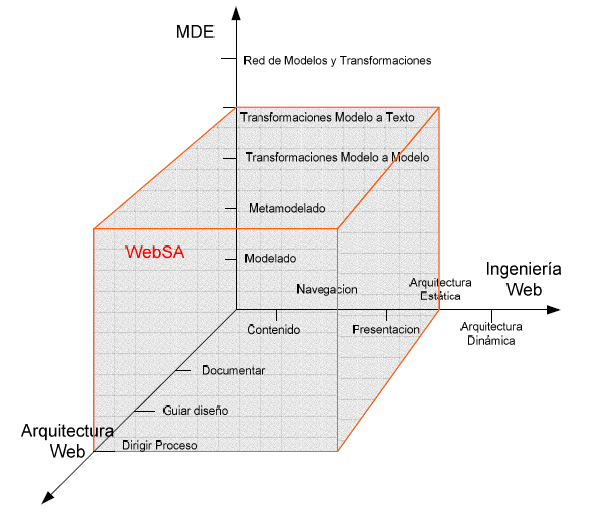
\includegraphics[scale=0.55]{Ch2/f1}
 % arqDHD.: 450x422 pixel, 72dpi, 15.88x14.89 cm, bb=0 0 450 422
\label{fig:planos}
\caption{Área de arqDHD dentro del campo de la arquitectura Web, las metodologías de diseño y su ingeniería} 
\end{center}

\end{figure}


\subsection{Área de construcción de la arqDHD} \label{secc:arqDHD_Situacion}


La Figura \ref{fig:planos} muestra una representación del espacio basada en
tres coordenadas, cada una de las cuáles representa una tendencia: \textbf{Ingeniería
Web} (eje: X), \textbf{Web} (eje: Z) y \textbf{MDE} (eje: Y). Situándose en un estado evolutivo dentro de cada coordenada o tendencia, arqDHD constituye el área dentro de la investigación donde se tomaron las decisiones para su diseño y creación. 

La \textbf{coordenada X} está representada por los conceptos de la Ingeniería Web y en ella se presentan las diferentes vistas que se han ido introduciendo a lo largo de su existencia y cómo las tres vistas funcionales son las primeras en
ser capturadas:
contenido, navegación y presentación. La cuarta vista, también capturada por
arqDHD, es la arquitectura estática. La única vista que no es representada por
arqDHD es la arquitectura dinámica, que representaría el comportamiento tanto
externo como interno de los componentes. Esta tarea no ha sido cubierta por el
presente trabajo.

La \textbf{coordenada Y} es ocupada por la \textbf{Ingeniería Dirigida por Modelos} (MDE) y en
ella se muestran los diferentes estadios por los que ha ido pasando:
representación de las vistas mediante modelos (modelado), formalización de los
modelos mediante el meta-modelado, definición de las transformaciones modelo a
modelo para establecer la traza entre los diferentes modelos del proceso y, por
último, las transformaciones modelo a texto que permiten obtener la
implementación a partir de los modelos.

En arqDHD se construyeron modelos orientados a la conexión de sistemas y artefactos que permitan un correcto ensamblado para lograr los requerimientos y el concepto del requerimiento de inyección de contratos que se viene enunciando. Queda sin embargo un largo
camino de interoperabilidad entre los modelos y transformaciones realizadas, que
permitan establecer una red para compartir los recursos definidos en MDE.


Por último, la \textbf{coordenada Z} la representa la \textbf{Arquitectura Web}. En ella se
muestra una serie de puntos que representan el papel que ha tenido la
arquitectura dentro de las aproximaciones. En un principio la arquitectura
únicamente se utilizaba para documentar. Poco a poco se ha ido extendiendo su
uso como guía para definir el diseño. El último estadio, que es el ocupado por
arqDHD, es aquel en el que la arquitectura define los artefactos más
importantes, dirigiendo el proceso de desarrollo


\section{El contrato como conector}

Entre la diversidad de propuestas de diseño de sistemas e-learning
con características adaptativas, existen diferentes variantes metodológicas y
tecnológicas, una de ellas es la incorporación de contratos context-aware. 

Conceptualizar al contrato como una componente de primera clase, donde las demás
componentes que lo relacionan dependen de su funcionamiento, nos brindará una
visión más completa orientada a la arquitectura y a la conexión entre sus
componentes.
Pensar el contrato como una pieza de conexión (referenciado con el término
“connectors”, conectores, en el área de arquitecturas en ingeniería de software)
nos permitirá incorporar (conectar) nuevos modelos independientes a los llamados framework e-learning.

En la figura \ref{fig:arqDHD1} representamos la integración de un modelo externo con
un framework e-learning por medio de un conector referenciado con el nombre
componente contrato. La componente modelo externo representa una entidad, puede ser un modelo
conceptual, una herramienta, applets, API (Application Programming Interface), o
cualquier sistema independiente que cumpla con la funcionalidad de brindar
información de contexto para ser incorporada en la semántica de la componente
contrato. Las herramientas y los servicios que componen el framework e-learning son
los puntos de comunicación con la componente contrato. Luego, la entidad sistema
representa el ambiente del servidor donde se encuentra el entorno de
la plataforma e-learning.

Este entorno abarca servidores web, servidores de base de datos, sistemas
operativos, archivos y repositorios de recursos, sistemas institucionales, etc.
La mayoría de los clientes deben ser estándares (similares a Web Browsers) y,
las salidas de las aplicaciones deben poder ser presentadas a los clientes
usando lenguaje de marcas tipo HTML.

En el próximo punto, nos centraremos en la importancia del tipo de modelado y
diseño con los que podríamos tratar a los contratos.


\subsubsection{Perspectiva de modelado}

 
El modelado y diseño de sistemas orientados a servicios complejos, no sólo
contribuye a una mejor comprensión de los problemas o posibles soluciones que se
pueden adoptar en un proyecto de I\&D como Obra Abierta, sino que facilita la
comunicación entre el grupo de investigación, especialmente cuando se encuentran
físicamente separados y/o afiliados a diferentes organizaciones.

El trabajo de modelado, es la base de procesos de desarrollo orientados a
servicios para educación y/o investigación, que deben guiar tanto a los
diseñadores como a los desarrolladores en el relevamiento de los requerimientos
pedagógicos y/o investigativos para implementarlos en un artefacto  -objeto- de
software. Esta tarea de modelado puede brindar una guía clara de trabajo al
equipo de I\&D, entregando las soluciones a tiempo y facilitando el logro de un
producto final de alta calidad, con bajos riesgos en el desarrollo.

Atendiendo a los cambios de la tecnología y a la continua evolución de
los estándares, el correcto modelado y diseño de soluciones Web complejas, se
torna cada vez más importante. Resultado de esto, es el nuevo paradigma
de desarrollo en sistemas llamado ”Model-Driver Architecture” (en adelante MDA).

El sistema MDA está focalizado en la importancia de los modelos de
plataformas independientes y plataformas específicas, que permiten una
separación de la abstracción del dominio de conocimiento del particular entorno
de implementación. En la actualidad, dependiendo de los objetivos de
las plataformas, con el desarrollo de herramientas avanzadas para el diseño a
partir de códigos de programación, el rol que cumple el modelo (o
modelado) comienza a ser fundamental. A través del uso de MDA, el modelo
representa a la programación de alto nivel construida para desarrollos de
aplicaciones como, por ejemplo, un dispositivo hipermedial dinámico como el de
Obra Abierta, con requerimientos factibles de trazar (en el sentido del modelado
desde el punto de vista de la Ingeniería de Software). Las herramientas
avanzadas pueden proveer generación automática de código XML, Java u otro código
de programación a partir de un determinado modelo. Un método correcto de
modelado debe brindar el soporte necesario para poder tomar la decisión sobre
qué parte de la aplicación debe ser expuesta como servicio o, qué parte de la
arquitectura debe ser confeccionada para invocar a los servicios Web.


El modelado de soluciones orientadas al servicio no es una tarea simple. Los
servicios heredan algunas características de sus predecesores – objetos y
componentes y también usan elementos del flujo de tareas y de los procesos de
negociación. De esta manera, el modelado de servicios debe cubrir totalmente las
diferentes facetas funcionales y tecnológicas para su prestación
e implementación. El uso de Lenguaje Unificado de Modelado (UML, por sus siglas
en inglés, Unified Modeling Language) como notación semi-formal para el modelado
de servicios es en la actualidad, una elección consensuada por la
comunidad informática.

Aunque en su origen, UML fue concebido para el modelado de sistemas orientados a
objetos, puede ser fácilmente extendido para soportar modelos de otros conceptos
tal como actividades de negocios, interfaces de usuarios y esquema de datos. Sin
embargo, podemos observar que, para el modelado orientado al servicio, todavía
este lenguaje se encuentra en una etapa inicial, ya que no ofrece mecanismos
para la representación de componentes y servicios a nivel lógico.


En Obra Abierta adoptamos estrategias y modelos basados en el concepto de
componentes de servicios que son similares a la propuesta de Zoran (2006), en su
publicación Modeling Services and Components in a Service-Oriented Architecture.
Una componente servicio es un bloque principal que interviene en algún tipo de
relación entre objetos del sistema, las componentes que conforman a los
servicios para educación y/o investigación son modeladas como contratos de
servicios en donde se efectúan algunos de los procedimientos pedagógicos o
investigativos (en forma de reglas) como ejecuciones de operaciones entre los
objetos.


El concepto de la componente contrato ha sido introducido en el capítulo
anterior, como una pieza de software que permitía la adaptación de servicios al
contexto de los objetos que lo utilizaban, o sea como componente para establecer
algún tipo de relación “controlada” entre ellos. En este capítulo, a los
contratos los abordaremos desde la perspectiva de los MDA, haciendo referencia
al propio modelo adoptado en Obra Abierta.


\subsection{Los conectores en entornos adaptativos}


\Section{Aspecto Dinámicos de la Arquitectura DHD}

Dichos sistemas son altamente dinámicos y muestran una estructura evolutiva.
Continuamente se añaden, eliminan o se reemplazan componentes, a veces incluso
como parte del funcionamiento normal. Estos detalles ya no son coyunturales,
sino estructurales y deben tenerse en cuenta durante el Diseño del sistema.
Por lo tanto, para ser realmente útil, un Lenguaje de Descripción de Arquitectura
(Adl) debe ser capaz de especificarlos. Sin embargo, esto no es lo normal en los
Adls existentes, cuya naturaleza es mayoritariamente estática. Los pocos que
muestran capacidades dinámicas muestran también limitaciones, que dependen en
gran medida de sus orígenes particulares.

Cuando la evolución de una arquitectura es continua y los cambios en su
interior siguen un patrón predefinido, entonces ha de considerarse que este
patrón forma parte intrínseca de la estructura. El objetivo de la Arquitectura
de Software es describir la estructura de los sistemas y, esto debería incluir
tanto a sus partes fijas o estáticas, como las partes cambiantes o dinámicas. De
hecho, en muchos sistemas, el rasgo diferencial, que lo distingue de otros
sistemas similares es el comportamiento dinámico de su arquitectura ya que a menudo,
puede resultar aún más importante que el esquema estático de partida. Algunos
ejemplos de sistemas para los que la definición de dinamismo es esencial son
los siguientes:

\begin{itemize}
 \item Los sistemas abiertos y distribuidos, cuya estructura cambia de manera
constante.

\item Los sistemas evolutivos de varias clases, que se ajustan a un cierto
patrón.

\item Los sistemas multi-agente (MAS), dentro y fuera del contexto
de Inteligencia Artificial y en general todos los sistemas capaces de expresar 
algún grado de movilidad.

\item Los sistemas reflexivos, que son interesantes en sí
mismos, pero que, además, constituyen la base de la propuesta final de este
trabajo.

\item Los sistemas continuos, de tiempo real y tolerantes a fallos, en los que
a menudo se requieren cambios, pero que no pueden ser detenidos para ser
actualizados.

\item Los sistemas adaptativos o auto-organizados, que modifican su propia
estructura para adaptarla a cada entorno concreto.

\end{itemize}


El DHD es parte de la última familia de sistemas enumerados, donde se permite
a través de una característica arquitectónica poder resolver requerimientos
funcionales, en este caso de adaptación, mediante la conjunción (conexión)
coordinada de subsistemas.


Hoy en día, todas estas propuestas han sido desarrolladas, y muchas otras se
han ido incorporando; muchos sistemas anteriores han sido adaptados o
reconocidos como Adls dinámicos, y se han desarrollado varias tesis doctorales
en todo el mundo [Cra97, MG99, Med99, dP99, Sch99, Wer99,Pry00, CV00] dedicadas
a este tema de algún modo. En definitiva, el desarrollo e interés creciente
de este campo es innegable, y se presenta, sin duda alguna, como uno de las
líneas de trabajo más fructíferas de la próxima década.


\section{Tipos de Dinamismo}

Todo sistema de software cuya estructura es descripta como una arquitectura tiene
siempre asociado algún tipo de comportamiento dinámico. Ahora bien, es
obvio que este dinamismo no siempre indica el mismo grado de variabilidad.
Algunos sistemas muestran una estructura inalterable, en la que los distintos
elementos se limitan a comunicarse. Otros sistemas, en cambio, muestran una topología interna que se altera continuamente e incluso se incorporan nuevos tipos de elementos.

Resulta fundamental, para poder realizar una comparación adecuada entre las
distintas aproximaciones, delimitar los diferentes tipos de dinamismo que
pueden aparecer en un sistema software.

La clasificación que se incluye más abajo ha sido planteada con este único
objetivo. No es exacta, ni pretende ser determinante ya que el límite entre las
distintas categorías puede aparecer difuminado en algunos casos. Sin
embargo, parece servir adecuadamente a su objetivo, esto es,
aclarar el tipo de actividad al que se hace referencia en cada casoy que ha
sido publicada en dos ocasiones [CFBSB00, CFBSB01].

Según esto, entonces, pueden identificarse los siguientes tres tipos de
dinamismo, en orden creciente de potencial para el cambio:

\begin{itemize}
\item 
Dinamismo Interactivo. Este término se refiere al movimiento de datos
entre componentes, el dinamismo inherente en la comunicación e interacción
usual. Se relaciona con cuestiones tales como la sincronización y los
protocolos afectando no solo a la estructura sino, también, al comportamiento de un sistema
computacional. Está presente de manera implícita en todo sistema, pero resulta
particularmente obvio en los concurrentes y paralelos.

\item
Dinamismo Estructural. Hace referencia a los cambios que afectan a los propios
componentes y sus interacciones, que normalmente se expresan como la creación
y destrucción de instancias y enlaces entre componentes. En este sentido, la
arquitectura de software del sistema resulta alterada, porque lo que cambia es
la estructura. Este tipo de dinamismo es natural en sistemas distribuidos.


\item 
Dinamismo Arquitectónico. Se refiere a los cambios en los tipos de
componente e interacción, modificando por lo tanto incluso el significado y el 
“vocabulario” del sistema. Se expresa como la inserción de nuevos tipos de
componente (y conector) y el borrado de algunos ya existentes. Ahora, lo que
cambia es la infraestructura, el sustrato en el que las arquitecturas se
definen, su meta-nivel. Este es el nivel definitivo de dinamismo y también el
más difícil de capturar y utilizar. Aún hay que demostrar su verdadera
importancia y utilidad, pero está claramente presente en los (auténticos)
sistemas abiertos.

\end{itemize}
\subsection{Reconfiguración Dinámica}

Hay al menos dos aproximaciones a la especificación de dinamismo en sistemas de
software. Una de ellas trata de encontrar un conjunto adecuado de comandos
imperativos, capaces de expresar cualquier configuración deseable. La otra
utiliza una sintaxis declarativa, que es generalmente más potente e intuitiva,
pero que no siempre tiene la flexibilidad deseada. El trabajo sobre este tema
se centró inicialmente en el primer enfoque; sin embargo, a medida que se
alcanza una mejor comprensión del dinamismo estructural, la presencia del
segundo tiende a aumentar.

A menudo, la denominación Arquitectura de Software Dinámica (ASD) ha sido
discutida. Muchos autores prefieren el término Reconfiguración Dinámica, que
ha sido consagrado por años de trabajo previo en el campo específico de la
configuración de sistemas distribuidos. Con esa expresión se hace referencia,
en general, a los cambios producidos en la topología de un sistema compuesto, igual a decir a cualquier alteración en el número y orden de los nodos y
los enlaces que lo constituyen. Lo cual es equivalente al grado de dinamismo que actualmente se
está alcanzando en los Lenguajes de Descripción de Arquitecturas. Según Jeff
Kramer, el nombre de Arquitectura Dinámica debería reservarse para referirse a
los sistemas en los que incluso el tipo de componentes implicados puede cambiar.
Este es, precisamente, el nivel de descripción al que se pretende llegar, por
lo que a lo largo de este trabajo esa expresión será utilizada a menudo, sin
mayores consecuencias.


\subsection{Tipos de Reconfiguración}

Hay varios tipos distintos de reconfiguraciones posibles, que manifiestan
problemáticas muy diferentes. Con el fin de determinarlas con mayor exactitud,
se han introducido una serie de clasificaciones. En este trabajo se mencionarán
dos de ellas, a saber:

\begin{itemize}
 
\item Según el tiempo. Uno de los aspectos críticos en un cambio es el
momento en que se produzca. La dificultad para realizarlo de manera adecuada
crece según se avanza en el proceso de desarrollo.

\begin{itemize}
\item Antes de la Compilación. Los cambios en la estructura prevista del
sistema se producen antes de su construcción, por lo que sólo hay que asegurar
su consistencia.

\item Antes de la Ejecución. El sistema ya ha sido elaborado, pero aún no
está funcionando, por lo que introducir un cambio sólo requiere, de nuevo,
asegurar la consistencia interna del sistema. Puede equipararse sin problemas
con el caso anterior.

\item Durante la Ejecución. Esta última es la auténtica Reconfiguración
Dinámica ya que los cambios se producen con el sistema en marcha: los componentes
tienen un estado y sus enlaces soportan cierto número de transacciones. La
problemática generada por este tipo de situaciones ha sido el campo de
investigación de la comunidad de configuración en los últimos diez años.
\end{itemize}

\item Según el origen. Es decir, según cómo se inicie el proceso y de acuerdo a quién tome la iniciativa, existen dos posibilidades que son las
que se detallan a continuación: 

\begin{itemize}

 \item Reconfiguración Programada. Reciben este nombre [EW92, MG99] las
operaciones que son iniciadas por el propio sistema, mediante una serie de
reglas proporcionadas como parte de su especificación. También, se ha mencionado
como reconfiguración restringida en tiempo de ejecución [Ore96], y es el
nivel de descripción que se desea alcanzar en la Arquitectura de Software.

\item Reconfiguración Ad-Hoc. Además de este nombre [EW92], ha recibido los
de reconfiguración evolutiva [MG99] o en tiempo de ejecución [Ore96]1. Hace
referencia a los cambios que son introducidos manualmente por el usuario y que,
por tanto, requieren en concurso de algún tipo de herramienta que haga
corresponderse a la arquitectura con un sistema real. Obviamente, no pueden ser
previstos, aunque en general sí pueden ser controlados.

\end{itemize}

\end{itemize}


La primera clasificación es obvia y ha sido planteada, entre otros, como autores del nivel de Wermelinger [Wer99]. La segunda clasificación, se debe inicialmente a los trabajos de Markus
Endler en Gerel [EW92], un lenguaje ligado a δarwin, pero que ha sido redescubierta
en múltiples ocasiones por otros autores; lo cual explica la gran variedad de
terminologías utilizadas.


\subsection{Operaciones Básicas de Reconfiguración}

Desde casi el principio, se ha determinado que toda configuración ha de poder
ser descripta en función de cuatro operaciones básicas, cuyo establecimiento
procede de Conic (§3.6.1). En realidad, no es muy difícil deducirlas de la
simple observación de un grafo, considerando en este caso al grafo como la
descripción más simple posible de la topología de cualquier sistema, en la
que los componentes se expresan como nodos y sus enlaces como aristas.

Las cuatro operaciones mencionadas son las siguientes:

\begin{itemize}

\item 
Crear (create). Se refiere a la creación de nuevos componentes.  Para ser
exacto, la instanciación de un nuevo ejemplar de un tipo de componente conocido. 

\item
Destruir (destroy). La inversa de la anterior: permite destruir un
componente ya
existente, eliminarlo del sistema.

\item
Enlazar (link). Crea un enlace simple entre dos elementos.

\item 
Desligar (unlink). La inversa de la anterior: destruye un enlace
preexistente.

\end{itemize}

Es importante aclarar que las ideas previas no significan que todo sistema de reconfiguración haya de tener
estas cuatro operaciones indicadas de manera explícita; al contrario, muchos
las expresan mediante estructuras declarativas y ni siquiera tienen
un equivalente claro para algunas de ellas. Lo que sí debe quedar claro es que toda reconfiguración, por compleja que sea, puede realizarse     
mediante la aplicación sucesiva de estas cuatro operaciones. Del mismo modo, si
un sistema no es capaz de expresar una transformación que, sin embargo, puede
ser descripta en función de estas cuatro operaciones, entonces puede afirmarse que el sistema no es
completo en lo que respecta a este tema. 

En realidad, estas operaciones proporcionan lo que aquí se ha denominado con el nombre de Dinamismo Estructural ya que, únicamente, permiten alterar la topología
del sistema. Sin embargo, constituyen lo que podría considerarse el límite
mínimo exigible a cualquier sistema que pretenda expresar arquitecturas
dinámicas. 

En los DHD el dinamismo está basado en la operación denominada Enlazar
(link). No obstante, a lo largo de la revisión podrá verse que hay dos
modelos conceptuales que predominan claramente por sobre cualquier otro; esto, no solamente es
cierto en los Adls dinámicos sino incluso en los más convencionales. 



\section{Descripción arquitectónica de los DHD} \label{secc:arqDHD}



En esta sección se presenta el modelo de arquitectura denominado arqDHD con un diseño adecuado para la implementación, configuración y posibles cambios en los procesos de inyección de contratos sensibles al contexto en entornos de eLearning originales (EeLO) \label{EeLO}. En la principal decisión de diseño se tuvieron en cuenta las atribuciones dinámicas que se persiguen y se seleccionaron cuáles serían los lugares apropiados para incorporar el ContratoDHD. 


\begin{figure}
\begin{center}
 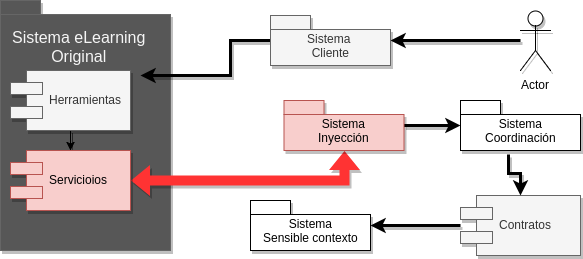
\includegraphics[scale=0.55]{Ch2/ArqDHD2.png}
\caption{Elementos arquitectónico involucrados en el proceso de inyección} \label{fig:arqDHD1}
\end{center}
\end{figure} 


La figura \ref{fig:arqDHD1} representa los elementos y las relaciones de una arquitectura que se tuvieron en cuenta. Por un lado, se parte de un sistema eLearning original reducido con las componentes “herramientas” donde se engloba la representación de todas las herramientas colaborativas (por ejemplo  una wiki, un foro, un examen, diversos recursos hipermediales, etcétera) que una determinada plataforma eLearning puede ofrecer a los usuarios finales. A su vez, se relaciona con la componente “servicio” encargada de representar las implementaciones de los métodos (funcionalidades) que ofrecen las herramientas que eventualmente pueden ser compartidas por varias de ellas (por ejemplo editar, consultar, publicar, borrar, aceptar, etcétera). Este tipo de relaciones es típico de los sistemas colaborativos web, manteniéndose como un estándar para este dominio de aplicaciones. 

Los otros elementos que aparecen en la arquitectura son dos sistemas que tienen relación directa con el sistema original. El primero es una representación para cualquier tipo de mecanismo de comunicación con las herramientas, particularmente en el framework Sakai \cite{sakaimanual} que estarían, a su vez, representadas las capas Presentación, Agregación y Clientes. El otro sistema conectado tendrá la responsabilidad de efectuar la inyección de los contratos sensibles al contexto. Esta relación está indicada con una flecha roja bidireccional para señalar que hay un importante flujo de mensajes de entrada y salida sobre la componente servicio. De esta manera, queda establecida un bloque de inyección entre la capa servicio, el subsistema de inyección y la relación bidireccional entre ellos. Entonces, la inyección se produce modificando únicamente la capa de servicio del framework original. En los capítulos que a continuación se presenta el desarrollo, se brindarán los detalles de diseño e implementación para esta relación.

Por otro lado, el sistema de inyección será el encargado de relacionarse con el sistema de coordinación de contratos que tiene la tarea de asegurar las propiedades dinámicas a la arquitectura. Específicamente, aquí se producen los reemplazos de contratos, a través de una nueva relación con el componente arquitectónico denominado \textbf{Contrato}, en el tiempo de ejecución configura el primer grado de adaptabilidad del sistema desde la arquitectura. La última relación, está dada entre el contrato y el sistema \textbf{Sistema Sensible al contexto} que se encargará de ofrecer la infraestructura necesaria para transformar al contrato en contrato sensible al contexto del DHD (ContextoDHD \ref{ContratoDHD}). 




\subsection{Diseño para la inyección}

En la publicación denominada \textit{" Investigación en el diseño y desarrollo para el enriquecimiento de
Un framework colaborativo web sensible al contexto "} (Sartorio et. al) \cite{inyecccion} aparecen los avances consolidados en el estudio-aplicación-desarrollo
de los aspectos fundamentales para el enriquecimiento de un framework web colaborativo con propiedades de sensibilidad al contexto
(FWCsc). Para este propósito se definió una estrategia y, en la presente sección, se expondrán los secretos de implementación y decisiones de diseños, que incluyó las siguientes acciones: 

Primero, desarrollando tareas de diseño, testing, documentación
de estilos arquitectónicos y especificación de una herramienta colaborativa web, teniendo en cuenta técnicas y metodología de desarrollo actuales. Segundo, implementación, instalación, configuración y soporte de una aplicación utilizando frameworks de desarrollo estándares. Tercero, consolidar ambientes y prácticas para el aprendizaje-enseñanza-investigación, colaboración y otros usos (compartir experiencia, vinculación con la comunidad de usuarios con intereses similares, K-12, Higher-Ed, Portfolios), en la construcción de espacios colaborativos web sensibles al contexto.

\subsubsection{Enfoque partiendo de Framework e-learnig originales}

La implementación de plataformas colaborativas constituye unos
de los medios más versátiles para el uso en actividades académicas. Un ejemplo que puede ser citado de este tipo de aplicaciones son: 
WebCT, BlackBoard, e-ducativa, Plataforma Mediáfora, Dokeos,
OfficeManager, Moodle, Nexus, ILIAS, Claroline.

Su constante evolución, crecimiento y adaptación permiten
tener cada vez mejores prestaciones y servicios. El eficiente uso
de estas plataformas implican tener sólidos conocimientos técnicos
para su instalación, mantenimiento y desarrollo. Al mismo tiempo
se debe contar con mı́nimas habilidades para la creación de los
distintos espacios de trabajos y definir las metodologı́as de uso.


En el marco de los análisis efectuados y teniendo en cuenta
experiencias de nuestro grupo de trabajo se sostiene que la incursión en
proyectos “open source“ con gran aceptación científica brinda una
de las propuestas más consolidadas de diseño y desarrollo de entornos colaborativos Web para educación, orientado a herramientas que se implementan a través de servicios comunes (denominados servicios bases). Por ejemplo, existen frameworks orientados a portales
donde el servicio de edición de mensajes es utilizado en herramientas tales como Foro, Anuncio, Blog, etcétera. Más aún, otra de las características salientes es la versatilidad para su extensión y/o configuración. En efecto, es posible alterar ciertas configuraciones
en tiempo de ejecución, por ejemplo, instrumentar una nueva funcionalidad en un servicio base.

Para este propósito se iniciaron estudios sobre la arquitectura y el diseño a partir de infraestructuras de aplicaciones e-Learning para la construcción y estudios de mejores técnicas de Especificación, Diseño, Modelado, Testing, Formalización y Documentación como aportes en el campo de la Ingenierı́a de Software. Además, es necesario definir y documentar adecuadamente el camino de construcción hacia  aplicaciones Web basadas en un framework colaborativo, con propiedades de sensibilidad al contexto y la utilización de contratos \cite{arqDHD21}



\susubsection{Punto de partida}

Los avances en las principales comunidades cientı́ficas sobre desarrollos de herramientas Web colaborativas permiten la participación
en varios niveles dentro de una activa comunidad de educadores, referentes institucionales y desarrolladores inspirados en las actividades de enseñanza, aprendizaje e investigación. Particularmente, los diseñadores y desarrolladores del proyecto Sakai \footnote{https://sakaiprojecto.org} trabajan conjuntamente con docentes y estudiantes profesionales de universidades internacionales. En este sentido, algunas de las universidades involucradas
en este proyecto son: Indiana University, University of Michigan, Yale University, Stanford University, Universidad Politécnica de Valencia y la Universidad del Valle de Guatemala. Todas ellas promueven la disminución de las distancias entre las necesidades del usuario final y el software. Ahora bien, debemos destacar que el mayor flujo de las actividades colaborativas se concentran en la lista de “e-mails”, “wiki”, “foros”, etc. Los miembros de estas comunidades presentan todo tipo de perfiles académicos e institucionales.


\begin{figure}
\begin{center}
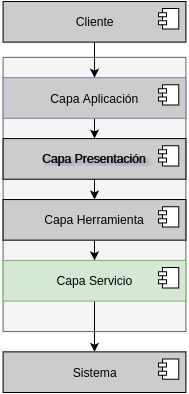
\includegraphics[width=2.5 in,totalheight=3 in]{Ch2/felo.png}
\caption{Elementos arquitectónico involucrados en el proceso de inyección} \label{fig:FeLO}
\end{center}
\end{figure} 


El punto de partida de esta experiencia se inicia con un diseño de arquitectura conceptual genérica a las que se ajustan los framework eLearning más populares. Luego, se identificarán los extractos de la arquitectura donde se representan los servicios de las herramientas. Se continúa con una propuesta de diseño que permita implementar el concepto de inyección referido en la sección \ref{secc:arqDHD}. Por último, se añaden nuevas componentes importantes de la arquitectura que complementan los aspectos adaptativos de los contratosDHD.  


El primer agregado al sistema web colaborativo original se produce a niveles de capas. El Framework Sakai está diseñado según una arquitectura de cuatro estratos de capas representada en la figura \ref{fig:FeLO}

La capa de \textbf{Agregación}, tiene la responsabilidad de las salidas de Sakai (y también aplicaciones externas a Sakai) que pueden ser combinadas utilizando una aplicación Servidor alojada aquí. Contiene un gestor de pantalla donde se controlan sus estados reales y ciertas transacciones de interfaz de usuario. Los soportes de accesibilidad son provistos por una combinación de interfaces de usuarios estándares esta capa y la de presentación.

La capa de \textbf{Presentación}, encargada de combinar los datos que provienen de las herramientas Sakai y las interfaces de usuarios creando metadatos al contenido que se brinda a los usuarios. Esta información es persistida externamente y será utilizada para poder analizar todas las experiencias a través de una herramienta Sakai denominada registro de actividades.  

La capa \textbf{Herramientas}, concentra la estructura de contenedores donde se encuentran la lógica de las funcionalidades que proveen las herramientas Sakai implementadas en los servicios y, también, las conexiones con la capa de presentación. Las herramientas atienden los pedidos de los usuarios y las respuestas a eventos del entorno, luego remite a los servicios adecuados y se encarga de proporcionar la respuesta a la capa superior.


La capa \textbf{Servicios}, interpreta a los servicios como una colección de clases que transforman datos para definir comportamientos. Estos datos pueden tener representaciones internas o ajustarse a los estándares de la comunidad industrial y/o científica. Las funcionalidades también pueden ser provistas a través de interfaces de aplicaciones (API). Un servicio puede invocar a otro servicio y creando dependencias. Los servicios son modulables y se ajustan a un diseño apropiado con el propósito de ser reusables y portables.

En los  capítulos precedentes se explicaron algunos de los fundamentos sobre el diseño de arquitectura a nivel arquitectónico. En esta sección de la investigación doctoral, se retoma la idea de inyección explicada anteriormente a nivel de arquitectura. Ahora, se propone un diseño para envolver los servicios del núcleo Sakai para el mecanismo de coordinación de contratos. De esta manera, se altera el diseño original del framework, agregando y modificando componentes que permitirán una mejor representación respecto a la inyección de información de contexto y el agregado de una nueva pieza de software que posee propiedades de sensibilidad al contexto mencionadas. Con este propósito, fue modificado el diseño de la capa de servicios original \cite{arqDHD17}, mediante una división en tres partes:


\begin{figure}
\begin{center}
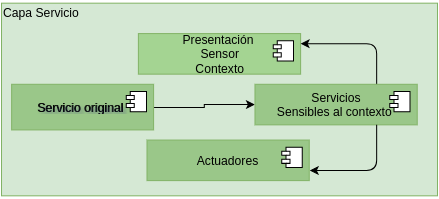
\includegraphics[scale=0.55]{Ch2/CapaServicio.png}
\caption{Elementos arquitectónico involucrados en el proceso de inyección} \label{fig:CapaServicio}
\end{center}
\end{figure} 



\begin{itemize}

\item \textbf{Servicios Originales:} Pertenecientes al núcleo del framework original, no afectados con el agregado del mecanismo
de coordinación de contrato.

\item \textbf{Servicios de Contexto:} Permite a clientes el acceso a en-
tidades, asignar, obtener y subscribir cambios en la información de contexto de las entidades.

\item \textbf{Servicios con coordinación de contratos (Servicios CSC):}
Servicios base del núcleo del framework Sakai modifica-
dos para poder efectuar la envoltura de los mecanismos de
coordinación.


\end{itemize}

Mediante la división del estrato servicios se puede interpretar a
los Servicios CSC como una nueva arquitectura basada en sistemas
estratificados[11]. Entonces, esta composición se efectúa por el estrato de coordinación de contratos y el estrato de cómputo. La capa
de cómputo estará compuesta por módulos de implementación (como por ejemplo los 
servicios Sakai previos a la incorporación de contratos). Mientras que la capa de coordinación estará compuesta por módulos
especı́ficos de coordinación, patrones tipo proxy y contratos.
La implementación de los Servicios CSC se realizarán utilizando un patrón de diseño de coordinación de contratos (”Coordination Contracts Design Pattern”) tomando como referencia
la propuesta de Fiadeiro \cite{arqDHD12, \cite{arqDHD13}. Este patrón está basado en el
patrón de diseño ”proxy” (o “Surrogate“) \cite{arqDHD14}. Por un lado, provee
una interfaz especı́fica (“SubjectInterface“), como una clase abstracta, para cada componente. Esta interfaz está conectada al programa real (”SubjectBody”) a través de un proxy dinámico reconfigurable. Por otra parte, soporta la reconfiguración dinámica del
código ejecutado por medio de solicitud de operaciones a través
del “proxy”.

El segundo subsistema está compuesto por una componente
contrato y su correspondiente mecanismo de coordinación. En este
caso, la coordinación del contrato se define como:
En términos generales, la coordinación de contratos es una
conexión establecida entre un grupo de objetos (en nuestras consideraciones los participantes serı́an un objeto cliente y un determinado servicio), donde reglas, normas y restricciones (RNR) son


\begin{comment}

\begin{figure}
\begin{center}
 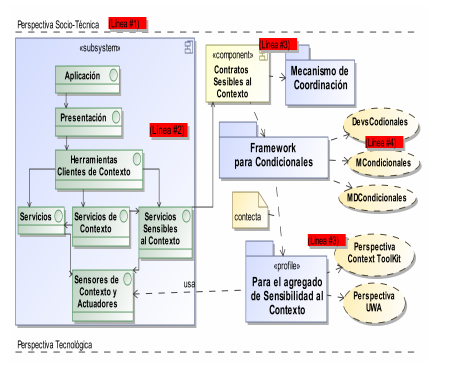
\includegraphics[scale=0.55]{Ch2/arqDHD_Implementacion.png}
 \caption{Arquitectura conceptual del DHD} \label{fig:arqDHD2}
\end{center}
\end{figure}

\end{comment}





superpuestas entre los actores participantes, estableciendo con un
determinado grado de control las formas de interrelación (o interacción).

El tipo de interacciones establecidas entre las partes es más
satisfactoria que las que se pueden lograr con UML o lenguajes
similares (orientados a objetos) debido a que éstas contienen un
mecanismo de superposición en el que se toman como argumento los
contextos. Cuando un objeto cliente efectúa una llamada a un objeto suministro, 
el contrato ”`intercepta”  la llamada y establece una
nueva relación teniendo en cuenta el contexto del objeto cliente, el
del objeto servidor e información relevante (respecto de la relación)
adquirida y representada como contexto del entorno. Como condición
necesaria, la implementación de los contratos no debe alterar el
diseño y funcionalidad en la implementación de los objetos.


El tercer subsistema corresponde a un framework implementativo “contex-awareness” que permite integrarse con algunas de las
componentes del primer subsistema para la recolección del censado de información de contexto. Luego, dicha información es
procesada a través de mecanismos que permitirán incorporarles
propiedades de sensibilidad al contexto. Su configuración fue resuelta a partir de las ideas fundadoras del trabajo de Dey sobre el
Context ToolKit \cite{arqDHD15} y el proyecto UWA \cite{arqDHD16}.

El cuarto subsistema lo compone un nuevo modelo pensado
para el diseño e implementación de condicionales que puedan ser
utilizados en la composición de reglas de contratos. La principal
idea de esta propuesta es estandarizar soluciones y brindar información necesaria en la creación de condicionales, donde su valores
de verdad deban se calculados a través de sistemas externos, como por
ejemplo, el tercer subsistema de la figura1. En este sentido,
los tipos de condicionales serán abstraı́dos en modelos que com-
prendan cálculos a partir de métricas, estructuras y simulación de
eventos discretos. También, puede verse a este subsistema como
integrador (conector) entre el subsistema de coordinación de con-
trato (segundo subsistema) y el sensible al contexto (tercer subsis-
tema).



\subsubsection{Áreas de integración}


A partir de \textbf{arqDHD} se comienzan a ordenar las cuestiones de diseños e implementaciones abordados en los siguientes capítulos. A lo largo de este recorrido se harán referencias directas e indirectas a todos los conceptos y enfoques abordadas en este capítulo. A su vez, se pueden identificar cuatro enfoques de interpretación y utilización de arqDHD. Cada una está relacionada con un conjunto de los elementos, relaciones y propiedades (de elementos y relaciones) de arqDHD. A continuación, se brindará una descripción conceptual que ponga en evidencia otros de los aspectos estructurales de nuestra propuesta de inyección de contratosDHD.


\begin{figure}
\begin{center}
 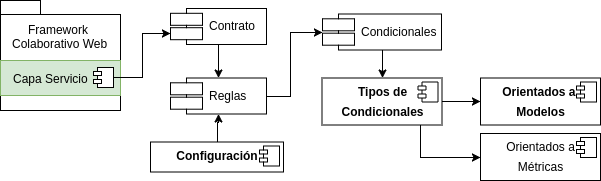
\includegraphics[scale=0.55]{Ch2/arqAreas.png}
 \caption{Áreas } \label{fig:arqAreas}
\end{center}
\end{figure}



Así como la arquitectura de la figura \ref{fig:arqDHD1} tiene definido los sistemas necesarios para la inyección, también fue necesaria definir áreas de integración en las que se pueda trabajar con herramientas y recursos externos en módulos para poder hacer incorporarlos de forma directa y con el menor costo de diseño e implementación posible. A continuación, se describen estas áreas con sus aportes para \textbf{arqDHD}.

\begin{enumerate}

\item \textbf{Área del estudio de arqDHD}
 
Este capítulo está dedicado a una propuesta de arquitectura para el DHD donde se tiene en cuenta varios aspectos arquitectónicos de los Framework eLearning originales y todos los elementos que intervienen en el proceso de inyección de los contratos. Principalmente, se tuvo en cuenta elementos, relaciones y las propiedades con alto impacto en el desarrollo e implementación. Para este propósito, se realizaron estudio de adaptación y aplicación de documentación de estilos arquitectónicos al framework web colaborativo Sakai con contratos sensibles al contexto \cite{arqDHD21}. Se proporcionan diferentes formas de interpretar la arquitectura Sakai con el propósito de construir una documentación adecuada a su comunidad de desarrollo \cite{arqDHD18}.

Luego, se propone una arquitectura ideal que describa la incorporación de contratos sensibles al contexto(CSC) utilizando estilos arquitectónicos y patrones de diseño. También, se persigue el propósito del agregado de propiedades de adaptación dinámica a los servicios bases del Framework Sakai. El esquema de la figura \ref{fig:arqAreas} define un mapa conceptual de las disposición de los elementos principales que se tuevieron en cuenta en la áreas denominada: ”Área del estudio de arquitectura y definiciones de arqDHD”. 


\item \textbf{Área de estudio de configuración de reglas de contratosDHD}
 
 
La configuración de las reglas de los contratos es una cuestión relevante para lograr adaptabilidad. Por este motivo, se tomaron como referencia obligada los trabajos de prueba de campo realizados en la tesis de la Dra. Soledad Ayala \cite{tesis:Soledad2014} quien analiza, desde una perspectiva socio-técnica, cómo se construyen las prácticas de lectura en el nivel educativo superior a través del uso de materiales educativos adaptados al \textbf{FWCsc}. A partir de los resultados de dicha investigación doctoral, obtuvieron protocolos e información necesaria para la construcción de reglas de contratos teniendo en cuenta diversos usos de las tecnologı́as considerando la compleja relación entre los aspectos sociales (de índole idiomática, cultural, educativa, legal, entre otros) y los aspectos técnicos de cada uno de los artefactos en particular y de los software en general.

Esto posibilitó ver cómo cada una de las distintas funciones
internas de las \textbf{FWCsc} se interrelacionan entre sı́, pero, principalmente, pensarlas en congruencia con la utilidad que los usuarios pueden otorgarles. En este sentido, la Dra. Ayala se pregunta acerca de cómo pueden identificarse y conceptualizarse los usos las tecnologías digitales desde un punto de vista epistemológico relativista de la tecnología. No hay un solo uso o un uso “correcto”, sino que coexisten usos adecuados, múltiples, correctos, orientados hacia ciertos fines, según el modo y los significados atribuidos por cada usuario. Cualquiera que estos sean, lo relevante de esta perspectiva es que permite analizar el vínculo entre los procesos de diseño y producción de las tecnologías y los diferentes usos que de los software, pero, además, posibilita al investigador interrogarse sobre los rasgos actuales que predominan en los usos referidos a las tecnologías digitales, el modo en que están siendo pensados, cómo se llevan a cabo, cuál es el estado de la cuestión y cuáles son los desafı́os presentes y futuros. 
El ámbito educativo es solo una arista fundamental de un campo que ya demostró en el desarrollo del hardware que el cielo es el lı́mite. Ahora bien, el análisis de los múltiples usos que realizan los diversos usuarios del otro lado de la pantalla”, del “cómo” los usuarios recuperan el diseño  y la arquitectura del programa, es uno de los mayores desafíos en las investigaciones referidas a la arquitectura de software. Queda por delante un desafı́o casi inacabable: recobrar la mirada del usuario, sus objetivos, pero por sobre todo, su forma de relación con la tecnologı́a y los rasgos de los procesos de interacción que co-construye con cada uno de los sistemas con los que interactúa, cualquiera que éstos sean. 


\item \textbf{Área de estudio sobre los condicionales.}

Esta área de estudio tiene el propósito de brindar un marco conceptual sobre la posibilidad de creación e implementación de condicionales adaptables al diseño y
propósito de los contratos sensibles al contexto. En la figura \ref{fig:arqAreas} está representado por las componentes \textbf{Condicionales} y su relación con \textbf{Reglas}.

En este caso, se propone un modelo de integración para conectar un subsistema que colabore con la configuración (cálculo) de los valores de verdad de las reglas de los contratos \cite{arqDHD19, arqDHD21}. Para este fin, se abordan líneas temáticas relacionadas con patrones de diseño, diseño de módulos y arquitectura de
software. Además, se plantean aspectos relacionados con la creación de metodologı́a y documentación específicas.

La figura \ref{fig:arqDHD2} representa una idea de la propuesta de diseño basada en los módulos que se deben tener en cuenta para concretar un diseño eficiente de  condicionales. En este caso, a partir de un módulo de integración \cite{arqDHD2} se concentran el control de las partes intervinientes. De esta manera, se define un módulo donde se efectúan los cálculos finales que determinan el valor de verdad del condicional.
Otro módulo es encargado de la recolección y toma de datos, extendiéndose para los casos particulares donde sea necesario contar con estructuras de árboles (como por ejemplo MDCondicionales \cite{arqDHD20}), aplicación de métricas (como por ejemplo MCondicionales \cite{arqDHD20}), expresiones lógicas, entre otras. Además, un módulo aparte se configura para describir todas las restricciones que deben cumplir el condicional, teniendo en cuenta su utilización dentro de las reglas de los contratos, con el propósito de no incurrir en contradicciones o inconsistencias con las “pre” y las “post” condiciones e invariantes. Las conexiones con otros subsistemas, por ejemplo, el sub- sistema sensible al contexto representado en la figura1, se encuentran encapsuladas en otro módulo de conexión. De esta manera, se implementa un  “callback” de un método perteneciente a la interfaz de un subsistema externo.

\item \textbf{Área de desarrollo e implementación de métricas para el análisis de las interacciones para el FWCsc}

En esta lı́nea se propone el desarrollo e implementación
de mejoras en las métricas para el análisis evaluativo de
la calidad de las interacciones en redes sociotécnicas mediadas por los \textbf{FWCsc} para la construcción y diseminación de conocimiento \cite{arqDHD1}. Estas métricas cuantitativas y cualitativas, son flexibles a los diversos requerimientos, tanto de los sujetos participantes como de las tecnologı́as sociales y digitales y se exponen atendiendo al marco teórico y metodológico de los Dispositivos Hipermediales Dinámicos\cite{arqDHD20}. En la figura \ref{fig:arqDHD} la componentes denominada \textbf{Orientados a Métrica} y \textbf{Tipos de Condicionales} establecen las estructuras que permitirán poder diseñar y construir condicionalesDHD donde sus grados de valor puedan ser inferidos a través de una métrica. Para este propósito, en los capítulos siguientes se presentará un diseño de aplicación de métricas a los contratos y, en particular, aplicaremos un tipo de condicional que deviene de la teoría de sistema complejo utilizando el formalismo DEVS (Discrete EVents dynamic Systems) para su modelado global y la integración tecnológica de dichas métricas.
También, sumamos el resultado obtenido en un caso de uso utilizando el entorno PowerDEVS. Así, la propuesta sienta las bases para el desarrollo de una herramienta de seguimiento
de procesos participativos que tienen como objetivo educar, investigar, producir y gestionar. A su vez, se obtiene un indicador para el cambio contextual de los participantes, resignificando una de las característica de sus comportamientos y atendiendo a la posibilidad de usar la información de interactividad como parámetro  “context-aware”  de los contratos. Al mismo tiempo, se consideró la posibilidad de establecer interfaces de conexión para ser utilizada como parte del cálculo de los valores de verdad de condicionales de las reglas en los contratos sensibles al contexto \cite{arqDHD2}.



\section{Conclusiones}

completar ...


